\documentclass[12pt]{article}   % artigo fonte 12
\usepackage[
a4paper,		% papel A4
left=1.5cm,		% margem esquerda
right=1.5cm,		% margem direita
top=1.5cm,		% margem superior
bottom=1.5cm		% margem inferior
]{geometry}
% Caracteres / Acentos / Português do Brasil
\usepackage[utf8]{inputenc}
\usepackage[T1]{fontenc}	
\usepackage[brazil]{babel}
% Pacotes Matemática
\usepackage{array,latexsym}
\usepackage{amsmath,amsfonts,amssymb,amsthm,mathabx,amstext}
\usepackage{dsfont}	% Conjuntos: $\mathds{N, Z, Q, R, C}$
\usepackage{graphicx}

\begin{document}
	\section{Acessibilidade versus cores}
		\par Quando usamos cores em ilustrações estatísticas, devemos nos preocupar em criar uma paleta de cores que seja acessível para daltônicos. Neste caso, devemos escolher cores que apresente alto contraste e que não haja sobreposição de cores que possam dificultar a compreensão da ilustração por daltônicos. Por exemplo, ao escolher as cores azul e roxo no gráfico à esquerda da Figura \ref{fig:azulroxo}, alguns leitores daltônicos verão tudo azul como o gráfico à direita da Figura \ref{fig:azulroxo}.
		
			\begin{figure}[h!]
				\centering
				\caption{Paleta azul, branco e roxo}
				\label{fig:azulroxo}
				\vspace{+12pt}
				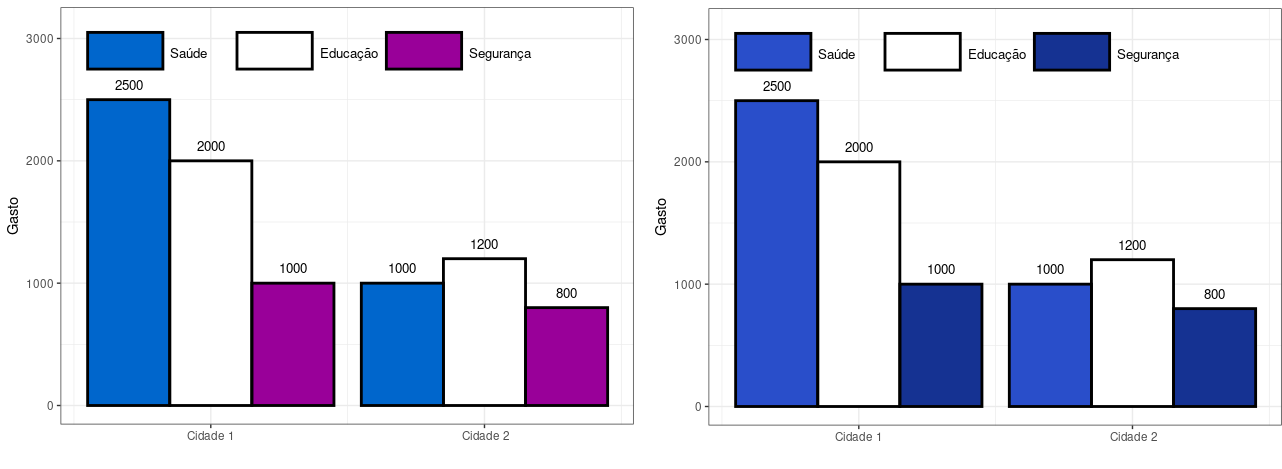
\includegraphics[scale=0.3]{AzulRoxo}
			\end{figure}
		\vspace{+16pt}
	
	    \par O mesmo ocorre com a escolha das cores verde e marrom na Figura \ref{fig:verdemarrom}. Existem vários tipos de daltonismo, sendo a deuteranopia o caso mais comum de daltonismo, que atinge $1\%$ da população masculina. Quem tem deuteranopia confunde verde, amarelo, vermelho e marrom, bem como, azul, roxo, azul água e rosa. Este é o problema na escolha da paleta de cores nas Figuras \ref{fig:azulroxo} e \ref{fig:verdemarrom}.
	    
	  		\begin{figure}[h!]
	    		\centering
	    		\caption{Paleta verde, branco e marrom}
	    		\label{fig:verdemarrom}
	    		\vspace{+12pt}
	    		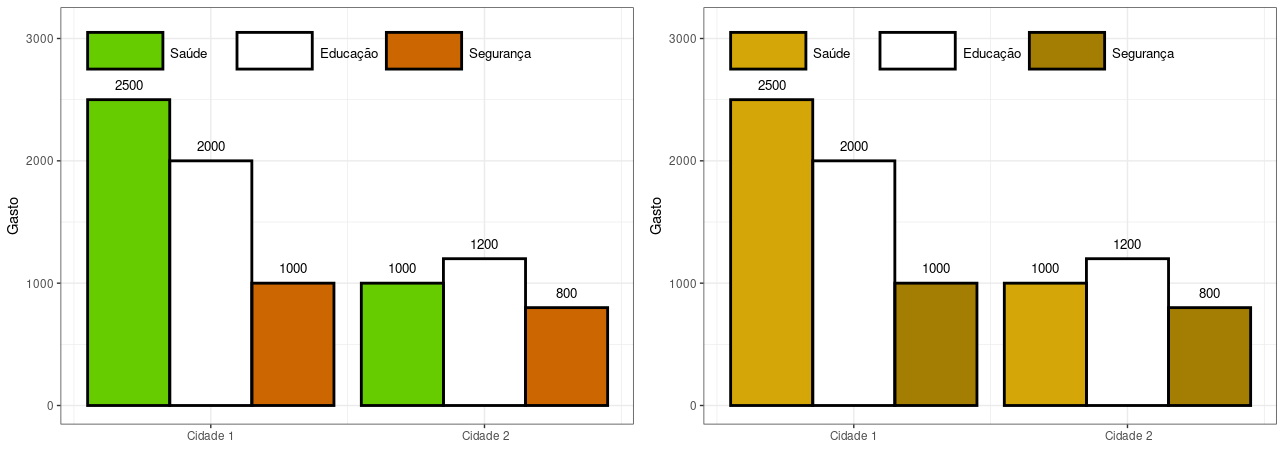
\includegraphics[scale=0.3]{VerdeMarrom}
	    	\end{figure}
    	\vspace{+16pt}
    
    	\par Para entender melhor o problema, vamos considerar os casos mais comum de daltonismo (informações obtidas da Wikipédia):
    	
    		\begin{itemize}
    			\item \textbf{protanopia}, quando há ausência na retina de cones 	"vermelhos", resultando na impossibilidade de discriminar cores no segmento verde-amarelo-vermelho do espectro.
    			\item \textbf{deuteranopia}, quando há ausência de cones "verdes", resultando, igualmente, na impossibilidade de discriminar cores no segmento verde-amarelo-vermelho do espectro.
    			\item \textbf{tritanopia}, quando há ausência de cones "azuis", resultando na impossibilidade de ver cores na faixa azul-amarelo.
    		\end{itemize}
    
    	\par Na Figura \ref{fig:paleta}, temos o espectro de cores normal (primeira faixa) e como essas cores são vistas por daltônicos com protanopia (segunda faixa), deuteranopia (terceira faixa) e tritanopia (quarta faixa). O caso mais grave e raro é a monocromacia, que ocorre quando o indivíduo apenas percebe a luminosidade, ou seja, ver apenas em uma escala de tons de cinza.
    	
    		\begin{figure}[h!]
    			\centering
    			\caption{Paleta com cores reais e como é vista por daltônicos}
    			\label{fig:paleta}
    			\vspace{+12pt}
    			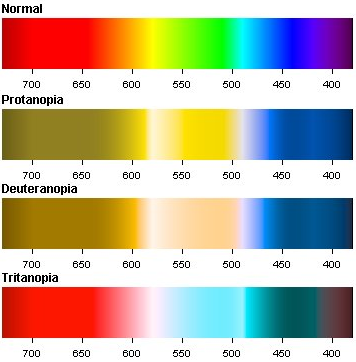
\includegraphics[scale=1.5]{paleta}
    		\end{figure}
    	\vspace{+16pt}
    	
    	\par Portanto, devemos tomar cuidado ao criar uma paleta de cores para gráficos. Um exemplo que funciona é o da Figura \ref{fig:azullaranja}. O recomendado é, sempre que possível, escolher uma cor na faixa que é vista como amarelo/vermelho pelos daltônicos e outra na faixa que é vista como azul/turquesa(azul água) para garantir o contraste.
    	
    		\begin{figure}[h!]
    			\centering
    			\caption{Paleta azul, branco e laranja}
    			\label{fig:azullaranja}
    			\vspace{+12pt}
    			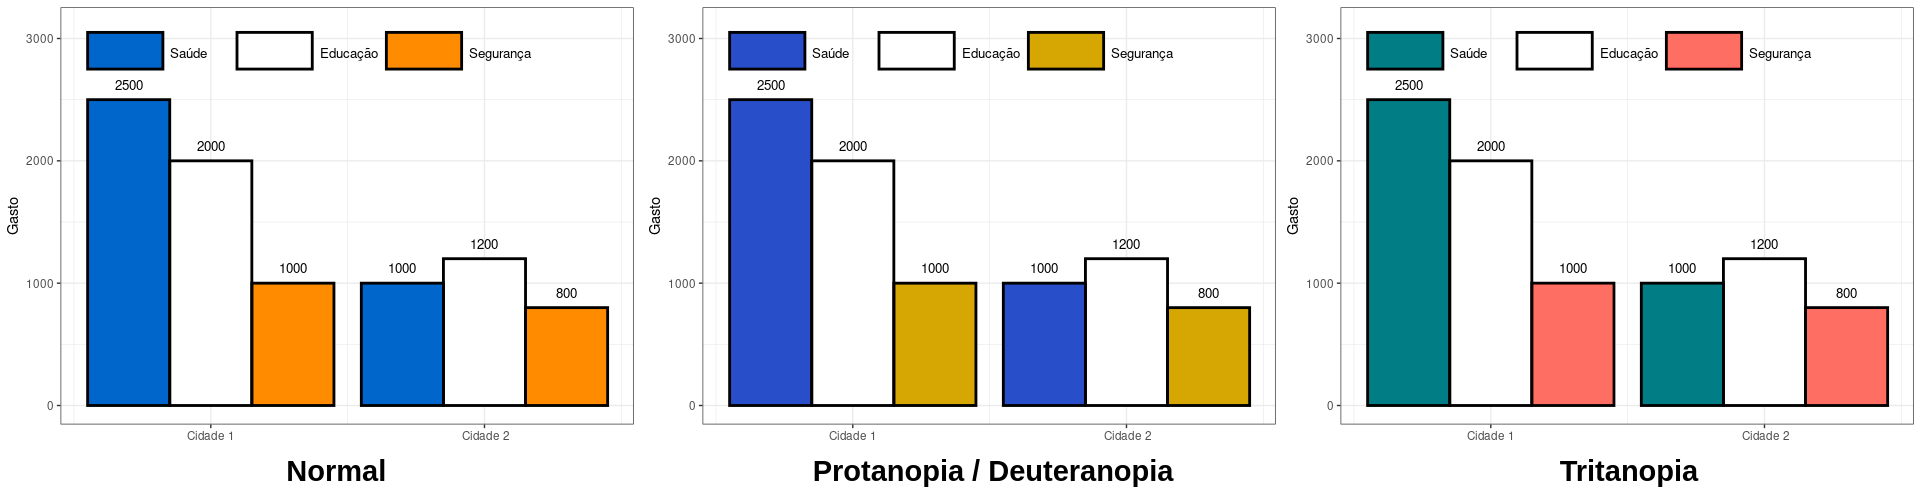
\includegraphics[scale=0.3]{AzulLaranja}
    		\end{figure}
    	\vspace{+16pt}
    	
    	\par O ponto crucial na questão do uso de cores é que, por mais que criemos uma paleta de cores com bom contraste para todos os tipos de daltonismo, ainda estamos usando cores. Quem tem daltonismo não consegue distinguir as cores por seus nomes e portanto, ao se referir no texto pelo nome da cor que está na figura, o daltônico provavelmente não vai entender. Portanto, a solução mais acessível é não confiar nas cores para seus trabalhos e projetos, mas sim, usar padrões. Pontos, traços em várias direções, larguras e espaçamentos, formas geométricas, símbolos e texturas passam a mesma informação e sem confundir daltônicos. Além disso, nada impede de usarmos cores quando também usamos padrões, como é o caso dos gráficos da Figura \ref{fig:padrao}.
    	
    		\begin{figure}[h!]
    			\centering
    			\caption{Exemplo de uso de padrões}
    			\label{fig:padrao}
    			\vspace{+12pt}
    			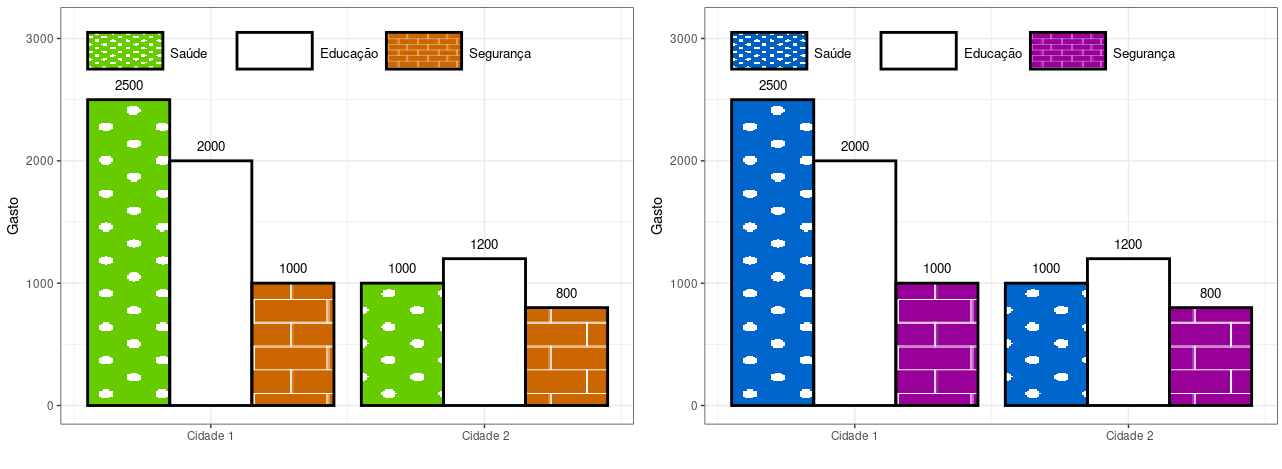
\includegraphics[scale=0.3]{padrao}
    		\end{figure}
\end{document}